\documentclass[12pt]{article}

\usepackage[english]{babel}
\usepackage[utf8x]{inputenc}
\usepackage{amsmath}
\usepackage{graphicx}
\usepackage{listings}
\usepackage{color}
\usepackage{pdfpages}
\usepackage{hyperref}
\vfuzz=3000pt
\title{Software Architecture Specification}

\makeatletter
\renewcommand{\@maketitle}
{
	\newpage
 	\null
 	\vskip 0em%
 	\begin{center}%
  	{\huge \bf \@title \par}%
 	\end{center}%
 	\par
} 
\makeatother

\begin{document}

%**************************************************************************
%  FRONT PAGE
%**************************************************************************

\maketitle

\vspace{4em}

\begin{center}%

  \LARGE {\bf Group 4}\\[2em]
  \LARGE {\bf Group Members:}\\[1em]
  \large
      Nico Taljaard			(10153285)	\\
      Neels van Rooyen		(29052735)	\\
	  Stephan Viljoen       (11008408)  \\
	  Martin Scoeman		(10651994)	\\
	  Jacques Lewis			(28183488)	\\
	  Uteshlen Nadesan		(28163304)	\\
	  Moeletji Semenya		(12349136)	\\[6em]
      
      {\bf Version 2.0}
    
\end{center}%

\newpage

%**************************************************************************
%  CHANGELOG
%**************************************************************************

\begin{tabbing}
\hspace*{2.5cm}\=\hspace*{2.5cm}\=\hspace*{7cm}\=\hspace*{3cm} \kill
03/03/2013 \> Version 1.0 \> Document Created \> Nico Taljaard\\
12/03/2013 \> Version 1.0 \> API UML Diagrams \> Neels van Rooyen\\
12/03/2013 \> Version 1.0 \> System Class Diagrams \> Nico Taljaard\\
12/03/2013 \> Version 1.0 \> Framework \& Technologies \> Stephan Viljoen\\
13/03/2013 \> Version 1.0 \> Database ERD \& Description \> Uteshlen Nadesan\\
13/03/2013 \> Version 1.0 \> Protocals \& Libraries \> Martin Scoeman\\
13/03/2013 \> Version 1.0 \> Sequence Diagrams \> Jacques Lewis\\
13/03/2013 \> Version 2.0 \> Added Diagrams \& Edited layout \> Nico Taljaard\\
13/03/2013 \> Version 2.0 \> UI Screen Designs \&  \>\\
						\>\> User Work-Flow Specification \> Moeletji Semenya\\
13/03/2013 \> Version 2.0 \> Finalized layout \& Structure \> Nico Taljaard\\

\end{tabbing}

\newpage

%**************************************************************************
%  TABLE OF CONTENTS
%**************************************************************************

\hypersetup{linktocpage}
\tableofcontents

\vspace{1.0cm}
\href{https://github.com/njTaljaard/Cos301_Phase2/}{Github}

\newpage

%**************************************************************************
%  INTRODUCTION
%**************************************************************************

\section{Introduction}

	\subsection{Purpose}

		\vspace{0.5cm}
		
		The purpose of this document is to declare and illustrate all lower levels of the system giving a more in-depth view of how the system should be implemented. This is done by designing UMLs, class diagrams and ERDs to depicted how each subsystem should be create as well as how the interconnection between components are to be create and utilized.

		\vspace{0.5cm}
		
	\subsection{Related Documents}

		\vspace{0.5cm}
		
		Master Requirement Specification: Provided by the University of Pretoria
		
		\vspace{0.5cm}

%**************************************************************************
%  SYSTEM DESCRIPTION
%**************************************************************************
\section{System Description}

		\vspace{0.5cm}
		
These software architecture design decisions are based on the constraints defined by the master requirement specification document:

		\vspace{0.5cm}
		
	\subsection{Technologies}
	
		\vspace{0.5cm}
	
		\indent\indent \textbf{Programming Languages}
		\begin{itemize}
			\item Python
			\begin{itemize}
			\item A high-level object oriented programming language that can be used for scripting,prototyping, testing and very easy to learn and implement.\\\\\\
			\end{itemize}
			\item HTML
			\begin{itemize}
			\item The system must be accessible to users and HTML Markup language will be used to for 	creating structured displayable content in a web browsers (Mozilla Firefox, Google Chrome, Apple Safari and Microsoft Internet Explorer). Reference 4.1.1.
			\end{itemize}
			\item CSS
			\begin{itemize}
			\item Used for formatting of HTML documents creating rich web interfaces.
			\end{itemize}
			\item JavaScript
			\begin{itemize}
			\item Dynamic programming language used for client side interaction.
			\end{itemize}
			\item SQL
			\begin{itemize}
			\item Used for data managing (insert, delete, update and read) of your relational data using the Object-Relational Mapper.
			\end{itemize}
			\item Java
			\begin{itemize}
			\item A Powerful language with vast libraries with which the android interface will be created. Reference 4.1.2
			\end{itemize}
		\end{itemize}
		
		\indent\indent\indent\linebreak\textbf{Application Server}
		\begin{itemize}
		\item A Django application server will be used to run and deploy the system within the cs.up.ac.za Apache web server. The webserver must be published as SOAP–based.
		
		\end{itemize}                                
		\indent\indent\indent\linebreak\textbf{Database Technology}
		\begin{itemize}
\item MySQL implement the quality requirements stated by the master specification and it decouples the system from the database. \\
			\item Scalability and Flexibility: \\
				Provides scalability, sporting the capacity to handle deeply embedded applications \\
				Platform flexibility (Linux, UNIX, Mac and Windows)
			\item Security \\
				Offering exceptional features that ensure absolute data protection when looking at database authentication, backup and recovery.
		\end{itemize}
		
		\vspace{0.5cm}
	
	\subsection{Frameworks}
	
		\vspace{0.5cm}
	
		\indent\indent \textbf{Object-Relational Mapper}
		\begin{itemize}
		\item A technique for converting data between incompatible types in object-oriented languages. With our application data to outlive the applications process. 
		The persistence to the relational database must be done using the Object-Relational Mapper bundled with Django. Django is the chosen Object-Relational mapper used to obtain, retrieve and transfer data between a variety of platforms such as from the MySQL database to the web client and android interface. You can define your data model in Python and access through the database API.
		\end{itemize}	
\indent\indent \textbf{Web Service Frame Work}
		\begin{itemize}
		\item The Django framework is based on the model view controller, which is used for creating complex database driven websites with the ability of reusability of components and rapid development. 
		The key quality requirements that Django accommodate are scalability, security, reliability and integration at a lesser extent.
		
		\end{itemize}	
		
		\vspace{0.5cm}
	
	\subsection{Protocols}
	
		\vspace{0.5cm}
	
		The protocols we will be using are HTTPS for security, LDAP for the \\ computer science web site, XML 		and JSON. \\
		\linebreak
		The two main protocols for data transfer in a web application environment are JSON and XML. We will be 	using JSON as our main data transfer \\ protocol, but also have support for XML. \\
		The reasons will be explained in accordance with the quality requirements.
		\\\linebreak
		 \textbf{Security:}
		\\\linebreak
		JSON in limited to storing only classical data like numbers and text, but with XML you can store any 		data type you want. That could be a security risk, because you can store an executable as well.
		\\\linebreak
		\textbf{Auditability:}
		\\\linebreak
		The simplicity of JSON and the fact that it’s only text base, makes it very easy to audit.
		\\\linebreak
		\textbf{Testability:}
		\\\linebreak
		JSON and XML are easy to test, because both of their implementation is self describing and is cross 		platform independent.
		\\\linebreak
		\textbf{Usability:}
		\\\linebreak
		Both XML and JSON is human readable, but JSON is more so. The reason is the JSON files are more 			restrictive and a lot less data formats that it supports. JSON uses an array to store data, where XML 		uses a tree. Seeing as arrays are more a structure of object oriented languages than trees are, it 			will be much easier the parse the data in the array than in the tree. 
		\\\linebreak
		\textbf{Scalability:}
		\\\linebreak
		Using a JSON document, without a schema makes it very easy to scale the JSON document. JSON also has 		no max size or max length of object. So you can send and receive a document without being depended on 		size. The limitations of the size will be determined by the server or browser. 
		\\\linebreak
		\textbf{Performance:}
		\\\linebreak
		The performance of JSON is very high, because of the fact it is only text base. So there will be no 		support for large files like images, videos and so forth.
		\\\linebreak\linebreak
		\textbf{Conclusion:}
		\\\linebreak
		JSON is selected as our main protocol, because it only supports text and no other formats. Seeing how 		our system will only be transferring text, JSON is the best option. Also JSON is simpler to use, 			easier to read and many people are changing from XML to JSON, because it is the newer technology.
				
		\vspace{0.5cm}
				
		\subsection{Libraries}
		\vspace{0.5cm}
		
		The libraries we will be using, will mostly if not all consist of open source libraries.
		\\\linebreak
		\textbf{PDF generator:}
		\\\linebreak
		The system must be able to generate PDFs on two different platforms, android and with a web service. 		For android we will be using the iText library that supports creating a PDF on android. For our server 	side, we will be using a PHP library called TCPDF, which will allow us to generate a PDF server side.
		\\\linebreak
		\textbf{JSON marshalling/de-marshalling:}
		\\\linebreak
		For our JSON marshalling/de-marshalling, we will be using the library EclipseLink MOXy. It works with 		XML, but also works great with JSON. There is a lot of support with this library, if one needed help.
		\\\linebreak
		\textbf{LDAP integration:}
		\\\linebreak
		We will be using django-auth-ldap 1.1.4 for the Django authentication backend that will authenticate 		against an LDAP service. For python we will be using the python-ldap library to allow us to use python 	to communicate with LDAP.

		\vspace{0.5cm}

%**************************************************************************
%  DETAILS OF SYSTEM
%**************************************************************************
\newpage
\section{Details of System}
	\vspace{0.5cm}
	
	\subsection{Class Diagram}
	\vspace{0.5cm}
	
	These diagrams depicts the classes that will be used with all the methods with parameters and return types and attributes to be used.
	
		\begin{figure}[htbp]
			\centering
			\fbox{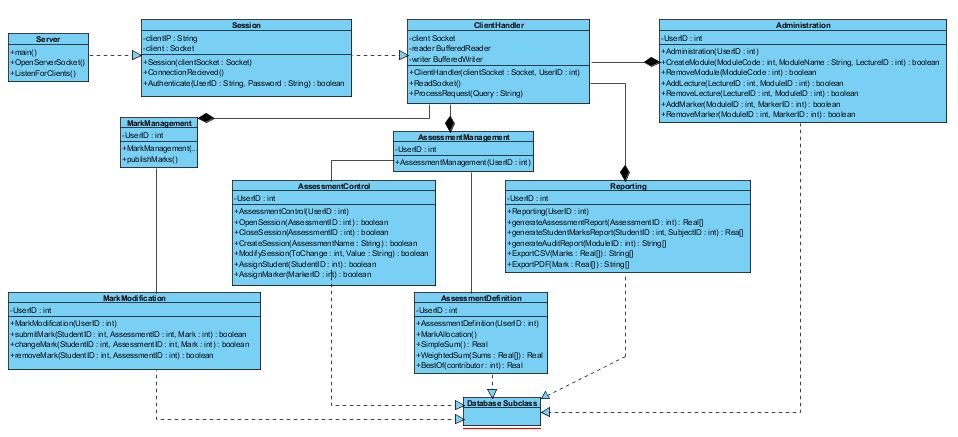
\includegraphics[width=15cm, height=7.5cm]{./Diagrams/System_ClassDiagram.jpg}}
			\caption{System Class Diagram}
		\end{figure}
		
		\begin{figure}[htbp]
			\centering
			\fbox{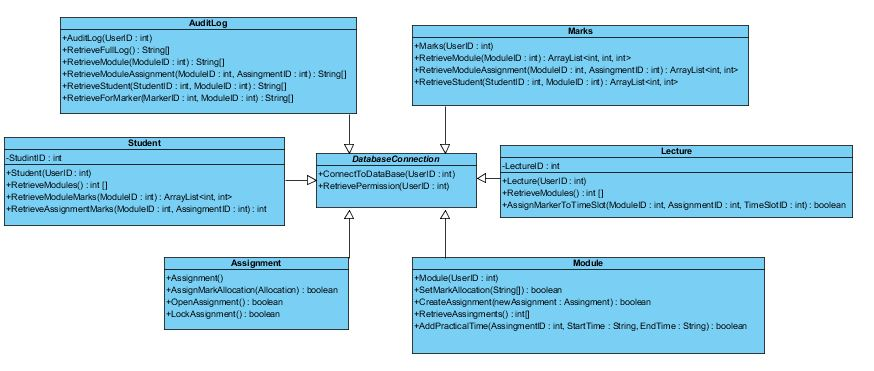
\includegraphics[width=15cm, height=3.5cm]{./Diagrams/Database_ClassDiagram.jpg}}
			\caption{Database Class Diagram}
		\end{figure}

	\vspace{0.5cm}
	\subsection{Database Design}
	
	\vspace{0.5cm}
	
		The Database software that is to be used is MySQL. The design above will be implemented in MySQL. The population of the database will be taken from the LDAP database of the Department of Computer Science. These will include, but not limited to, student numbers, names, surnames, courses, lecturers’ details, etc. 
		
		\begin{figure}[htbp]
			\centering
			\fbox{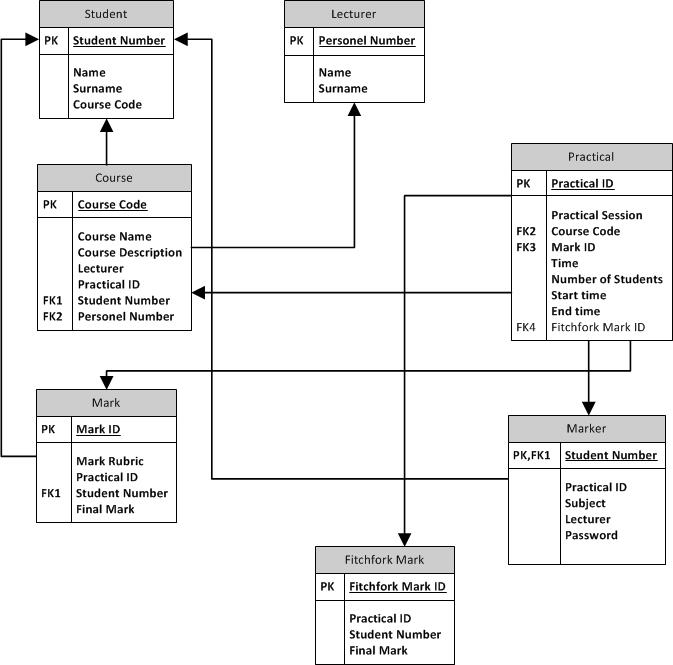
\includegraphics[width=15cm, height=12cm]{./Diagrams/Database.jpg}}
			\caption{Database ERD}
		\end{figure}
		
		\vspace{1.5cm}
		
		\begin{itemize}
			\item{Student}
				\begin{itemize}
				\item All student details will be imported and added to complete the student table of the database. All students have a unique student number that identifies them, names, surnames and courses can then be added. Adding these details will enable access to all additional tables.
				\end{itemize}
			
			\item{Practical}
				\begin{itemize}
				\item The Practical table has the session for that specific practical the number of students assigned to that practical, the Fitchfork marks that can be added although it is not mandatory. The start and end times are also added as they are essential for the application to know when to open and close editing of the database. The practicals are indirectly linked to the lecturers who will have access to their subject’s practicals.
				\end{itemize}
			
			\item{Mark}
				\begin{itemize}
				\item A table of marks will capture the marks for each student along with the final mark each student will receive for the practical. Marks are linked to the student and the practical itself via the student number and practical identification number. This will simplify access, not only for the students, but also for the markers and lecturers combined.
				\end{itemize}
			
			\item{Marker}
				\begin{itemize}
				\item Markers are in a separate database and include a password specific to that marker for accessing the android application and include the overseeing lecturer and subject and practical the marker is assigned to.
				\end{itemize}
			
			\item{Fitchfork}
				\begin{itemize}
				\item Marks that need to be imported from Fitchfork will be done separately and then added to the above database tables to complete the database entries for the practical. \\
				\end{itemize}
			
			\item{Lecturer}
				\begin{itemize}
				\item All courses that require marks to be entered into this database will have a lecturer assigned to the course and hence, the practical.
				\end{itemize}
		\end{itemize}
	
	\vspace{0.5cm}
	\subsection {Logic View}
	\vspace{0.5cm}
		
		\begin{figure}[htbp]
			\centering
			\fbox{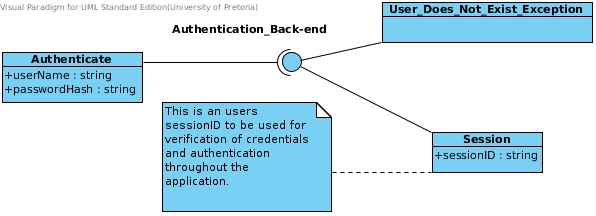
\includegraphics[width=12cm, height=4cm]{./Diagrams/Authentication_API.jpg}}
			\caption{Authentication API}
		\end{figure}
				
		\begin{figure}[htbp]
			\centering
			\fbox{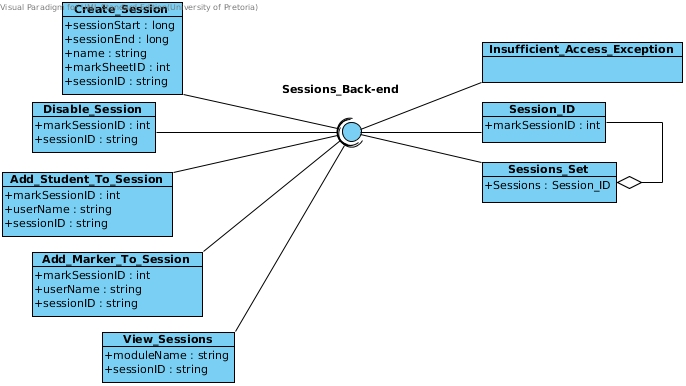
\includegraphics[width=12cm, height=5cm]{./Diagrams/Sessions_API.jpg}}
			\caption{Sessions API}
		\end{figure}
			
		\begin{figure}[htbp]
			\centering
			\fbox{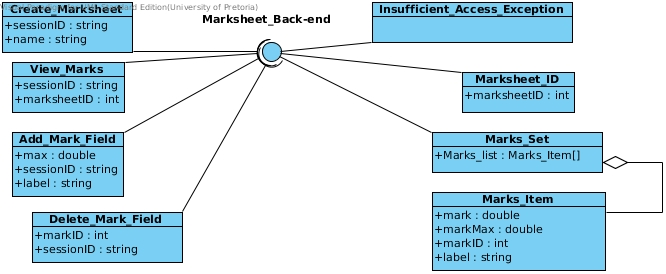
\includegraphics[width=12cm, height=4cm]{./Diagrams/Marksheet_API.jpg}}
			\caption{Marksheet API}
		\end{figure}
				
		\begin{figure}[htbp]
			\centering
			\fbox{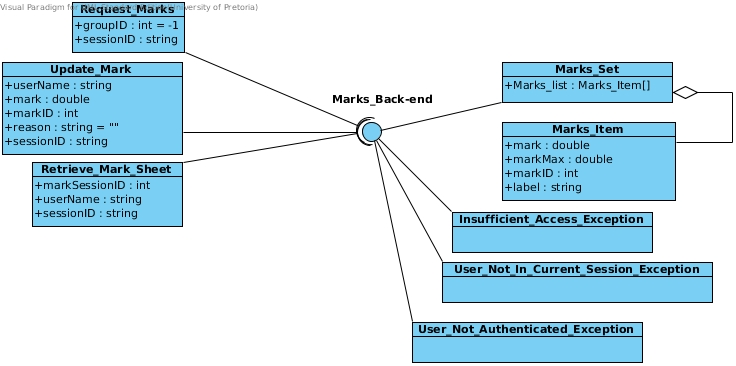
\includegraphics[width=12cm, height=4.5cm]{./Diagrams/Marks_API.jpg}}
			\caption{Marks API}
		\end{figure}
		
		\begin{figure}[htbp]
			\centering
			\fbox{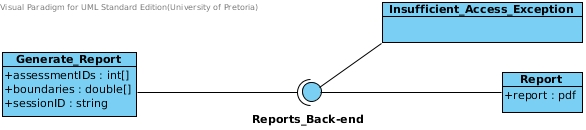
\includegraphics[width=12cm, height=4cm]{./Diagrams/Reports_API.jpg}}
			\caption{Reports API}
		\end{figure}
		
	\vspace{0.5cm}
	\subsection {Sequence Diagram}
	\vspace{0.5cm}

		\begin{figure}[htbp]
			\centering
			\fbox{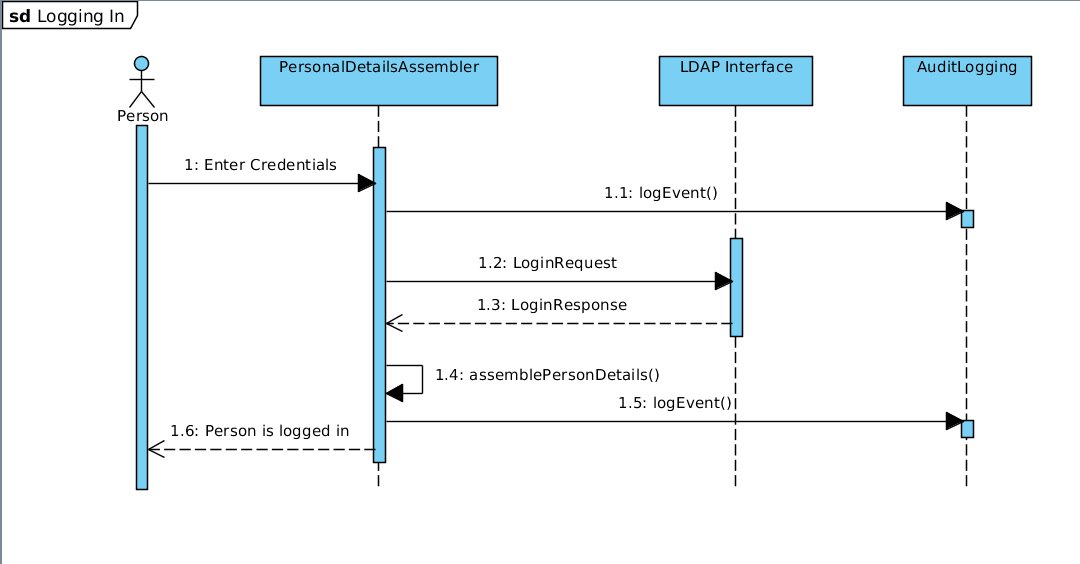
\includegraphics[width=15cm, height=5cm]{./Diagrams/sd_LoggingIn.jpeg}}
			\caption{Login}
		\end{figure}
		
		\begin{figure}[htbp]
			\centering
			\fbox{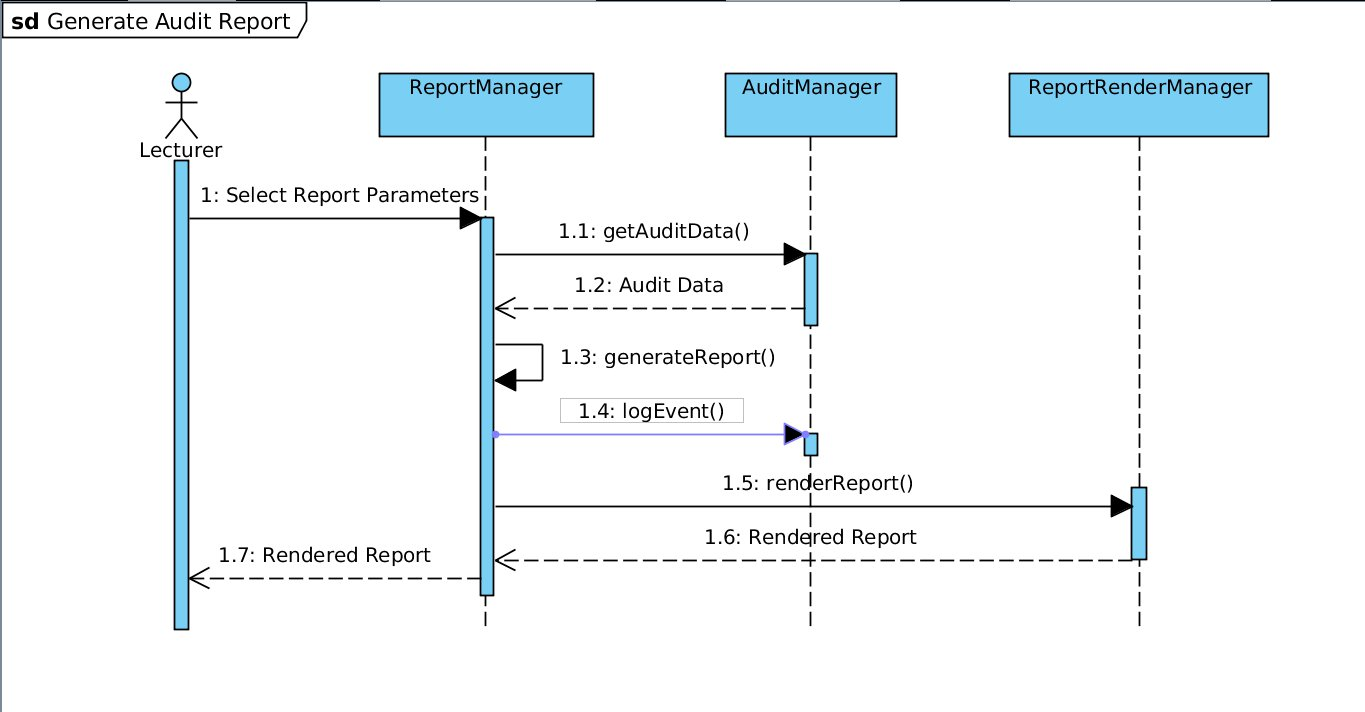
\includegraphics[width=15cm, height=5.5cm]{./Diagrams/sd_GenerateAuditReport.jpeg}}
			\caption{Generate Audit Report}
		\end{figure}
		
		\begin{figure}[htbp]
			\centering
			\fbox{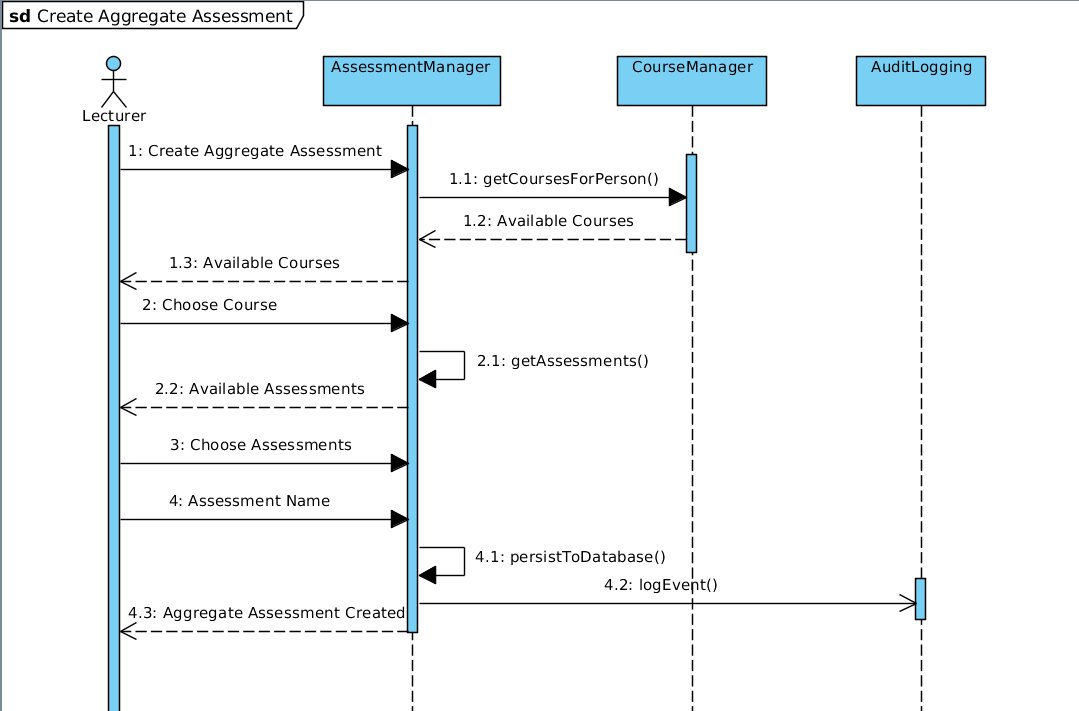
\includegraphics[width=15cm, height=7.5cm]{./Diagrams/sd_CreateAggregateAssessment.jpeg}}
			\caption{Create Aggregate Assessment}
		\end{figure}
		
		\begin{figure}[htbp]
			\centering
			\fbox{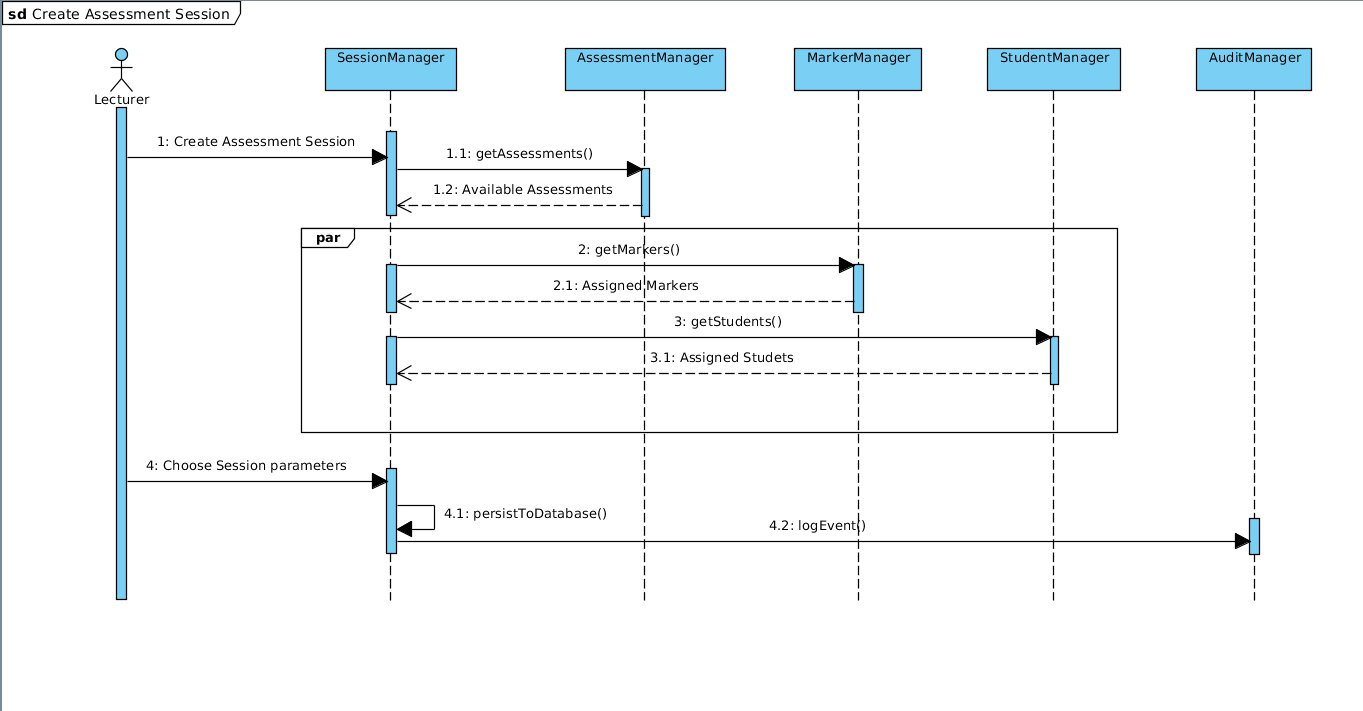
\includegraphics[width=15cm, height=7.5cm]{./Diagrams/sd_CreateAssessmentSession.jpeg}}
			\caption{Create Assessment Session}
		\end{figure}
		
		\begin{figure}[htbp]
			\centering
			\fbox{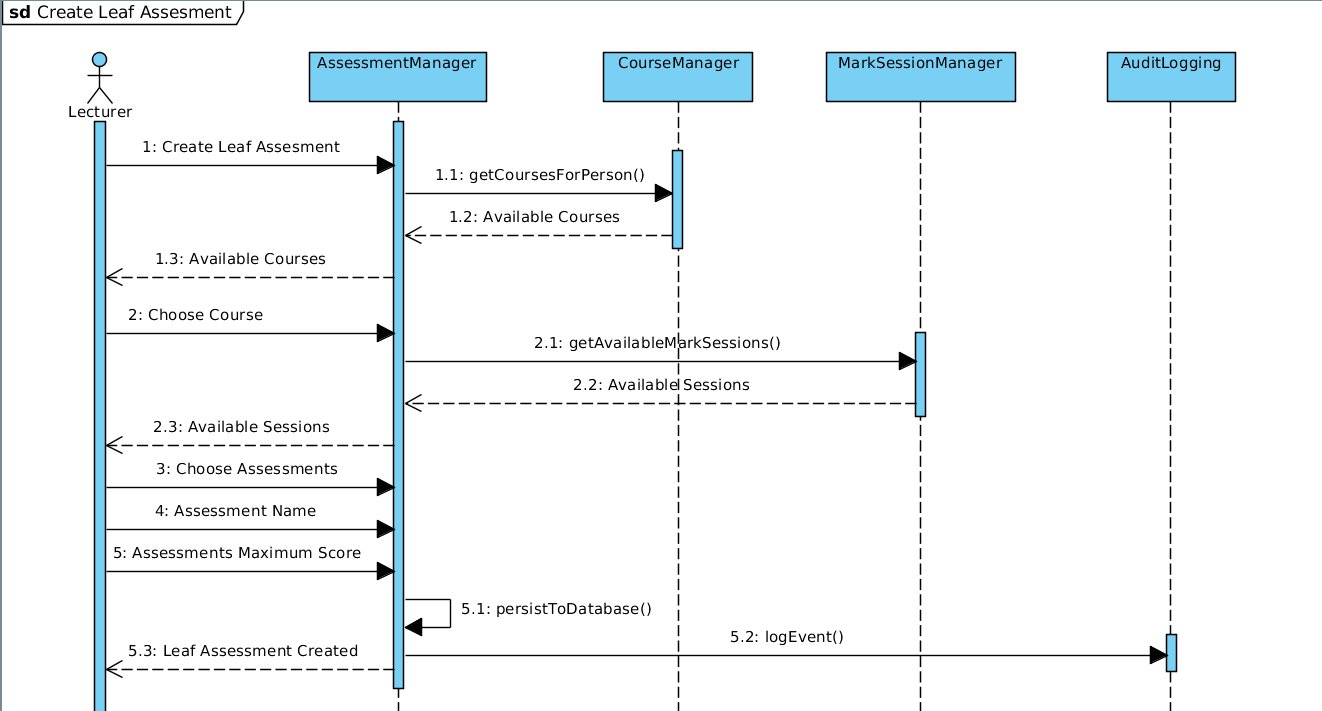
\includegraphics[width=15cm, height=6.5cm]{./Diagrams/sd_CreateLeafAssessment.jpeg}}
			\caption{Create Leaf Assessment}
		\end{figure}
		
		\begin{figure}[htbp]
			\centering
			\fbox{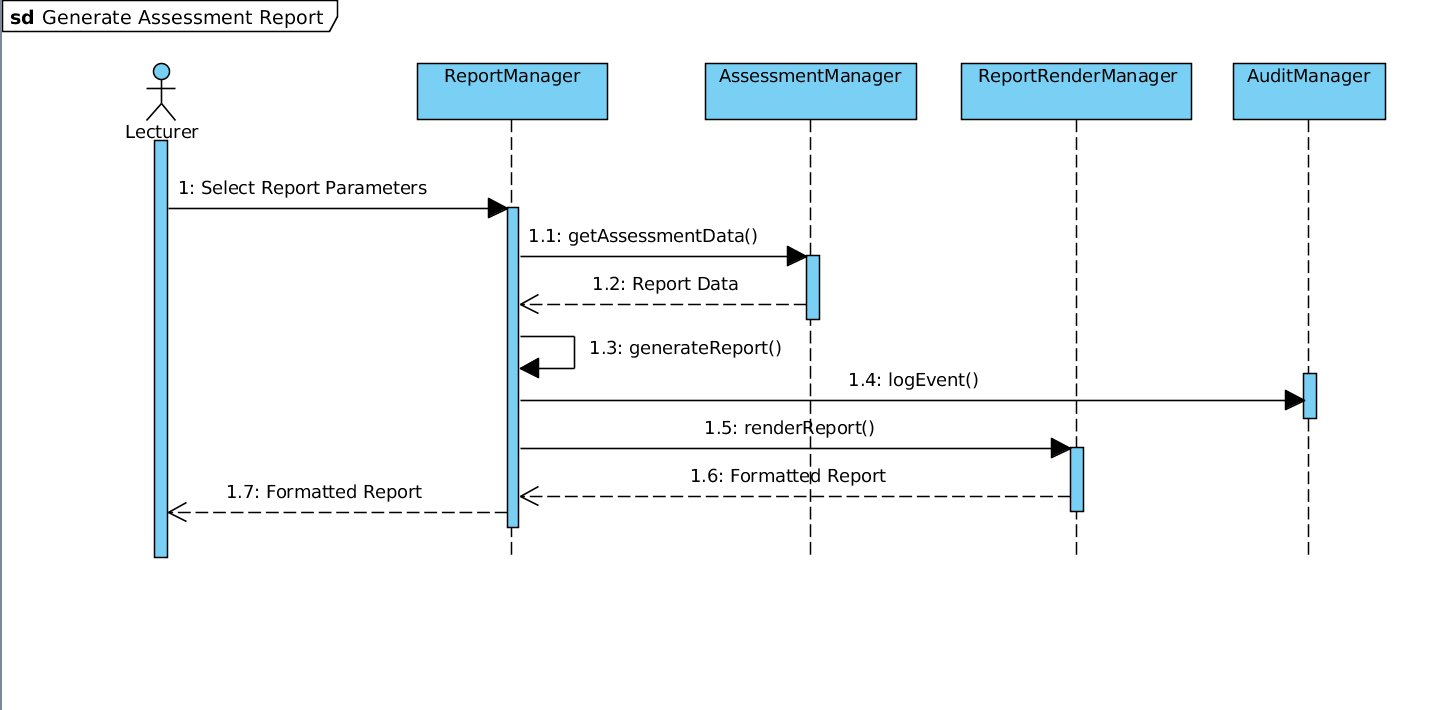
\includegraphics[width=15cm, height=6.5cm]{./Diagrams/sd_GenerateAssessmentReport.jpeg}}
			\caption{Generate Assessment Report}
		\end{figure}
		
		\begin{figure}[htbp]
			\centering
			\fbox{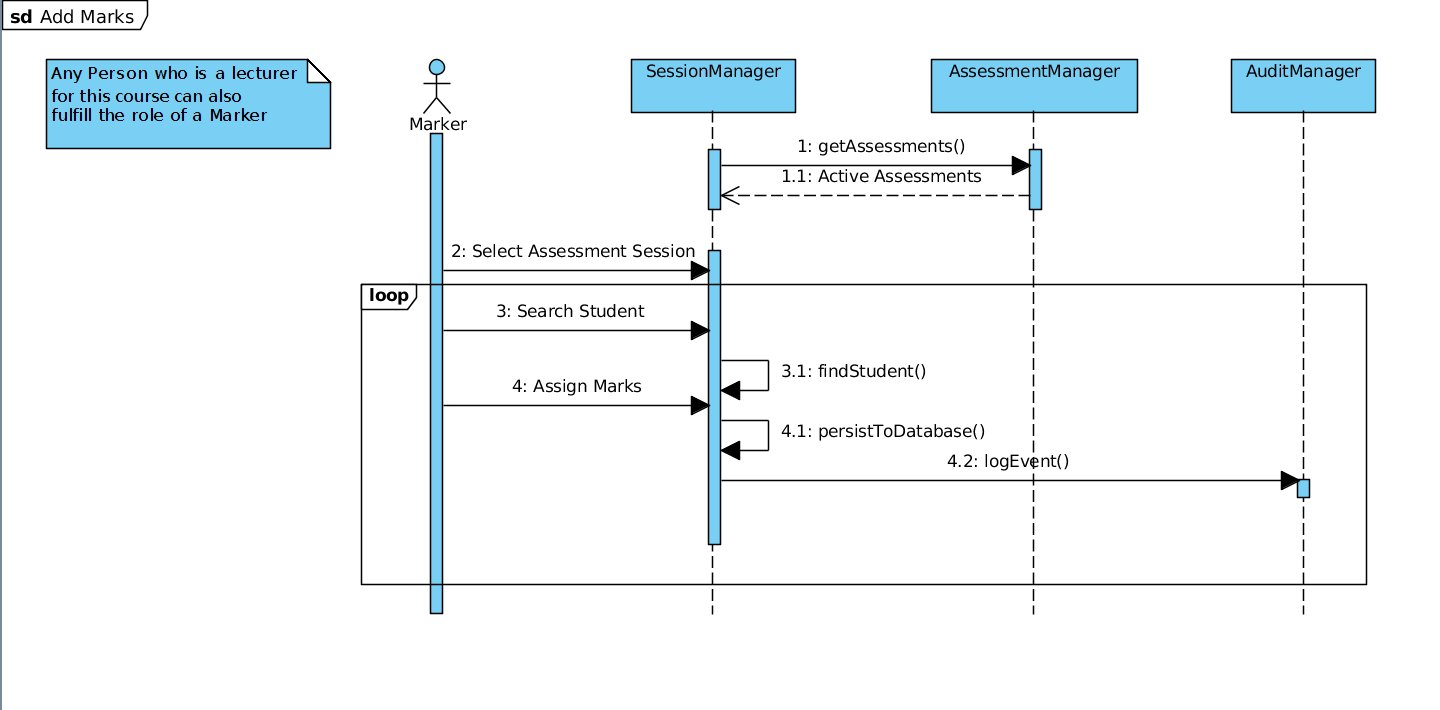
\includegraphics[width=15cm, height=6.0cm]{./Diagrams/sd_AddMarks.jpeg}}
			\caption{Add Marks}
		\end{figure}
		
		\begin{figure}[htbp]
			\centering
			\fbox{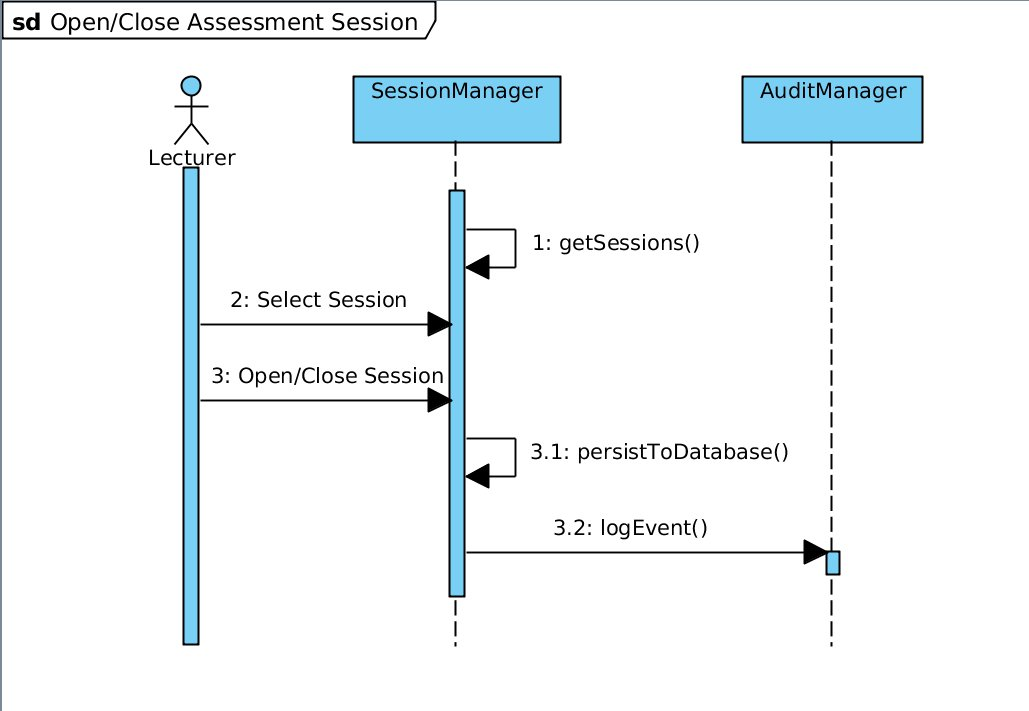
\includegraphics[width=15cm, height=6.0cm]{./Diagrams/sd_OpenCloseSession.jpeg}}
			\caption{Open Close Session}
		\end{figure}

	\newpage
	\section{UI Screen Designs and User Work-Flow Specification}
	
		This section will look at how the system will be used by the different users. Each functional requirement will be accompanied by the appropriate screen designs(The web and mobile user interfaces). 

	\subsection{Log In}
		\begin{figure}[htbp]
		\centering
		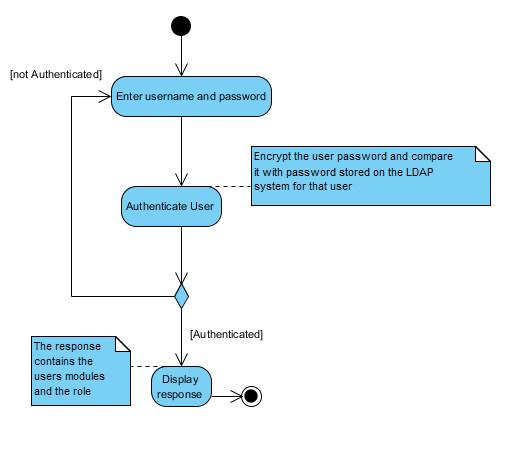
\includegraphics[width=0.7\linewidth]{./Diagrams/uml_login}
		\caption{User log in activity diagram.}
		\label{fig:uml_login}
		\end{figure}
	
	The activity diagram above is a abstract depiction of what will happen when a user logs into the system. After the user gets authenticated by the system, the authentication response object will contain the users information(the modules and roles) as shown in Figure 3 and 5.
	
	\pagebreak
	
	\subsubsection{Mobile Interface Screen Designs}
	
		\begin{figure}[htbp]
		\centering
		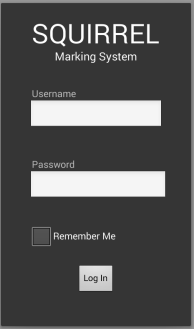
\includegraphics[width=0.7\linewidth, height=12cm]{./Diagrams/mobile_login}
		\caption{The mobile log in screen design.}
		\label{fig:mobile_login}
		\end{figure}
	
	\pagebreak
	
		\begin{figure}[htbp]
		\centering
		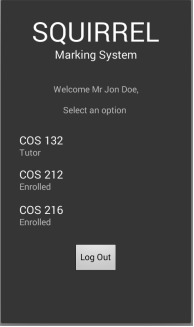
\includegraphics[width=0.7\linewidth, height=12cm]{./Diagrams/mobile_welcomeScreen}
		\caption{Screen design of a successfull log in request.}
		\label{fig:mobile_welcomeScreen}
		\end{figure}
		Figure 3 shows the modules the user is associated with and the roles users have for particular module. 

	\pagebreak
	
	\subsubsection{Web Interface Screen Designs}
	
		\begin{figure}[htbp]
		\centering
		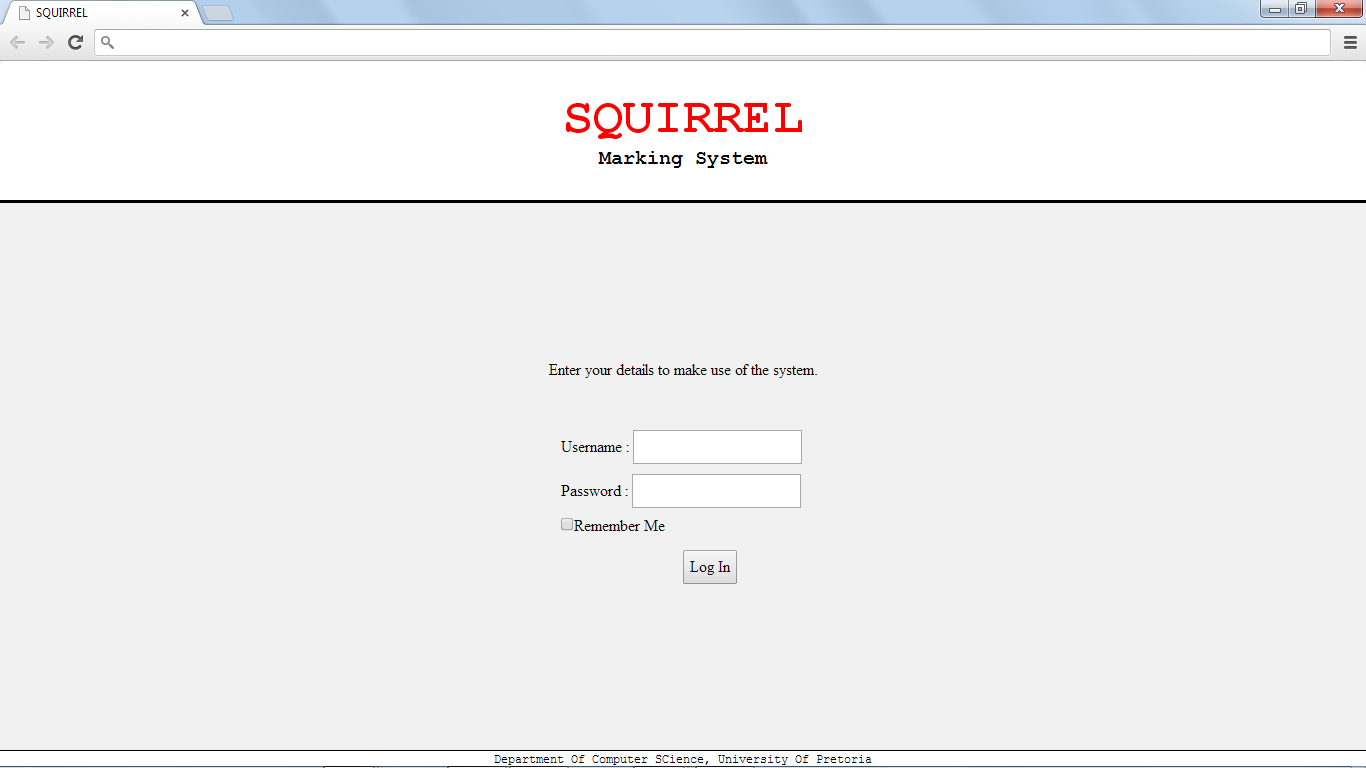
\includegraphics[width=1.0\linewidth]{./Diagrams/web_login}
		\caption{Screen design for web interface}
		\label{fig:web_login}
		\end{figure}
			
		\begin{figure*}[htbp]
		\centering
		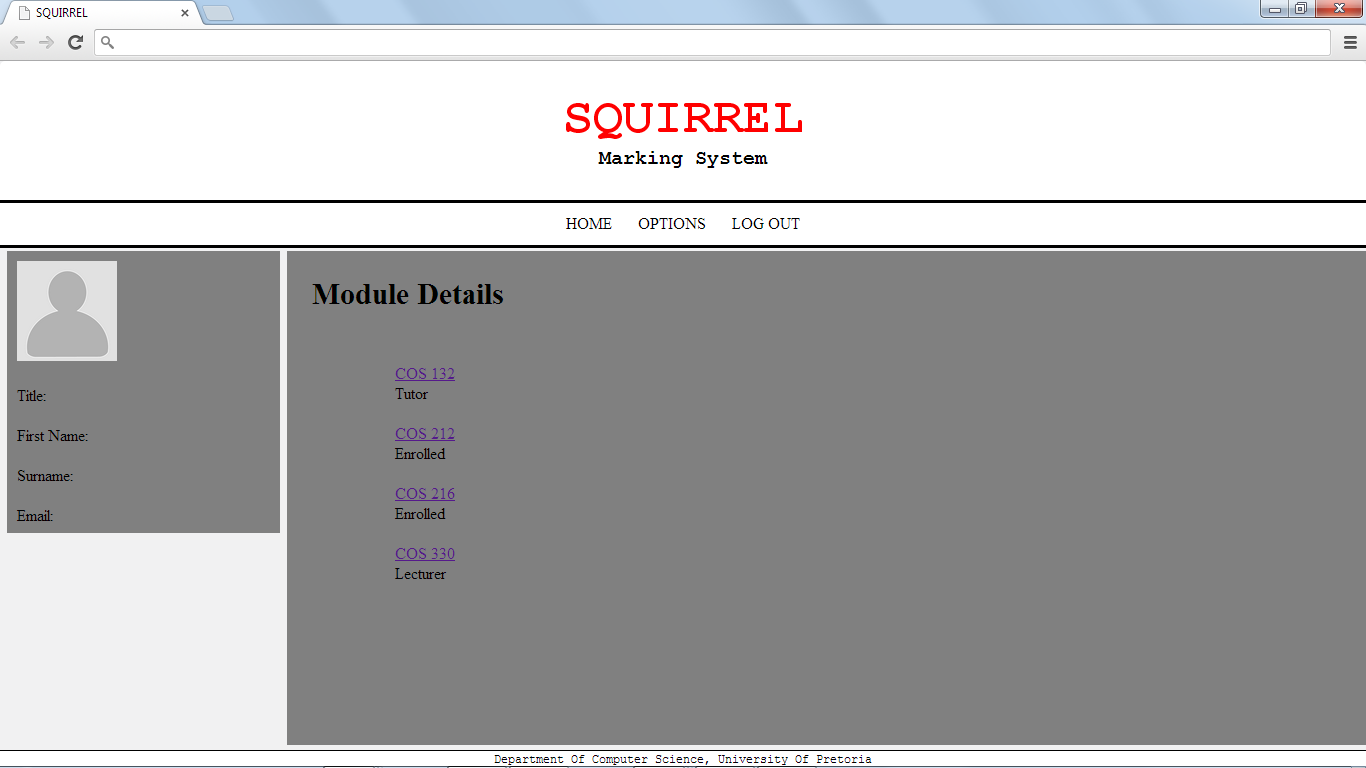
\includegraphics[width=1.0\linewidth, height=12cm]{./Diagrams/web_modules&roles}
		\caption{This is the welcome page the user sees after successfully being authenticated.}
		\label{fig:web_modules&roles}
		\end{figure*}
	
	\newpage
	\subsection{Assessment Creation}
	
		\begin{figure}[htbp]
		\centering
		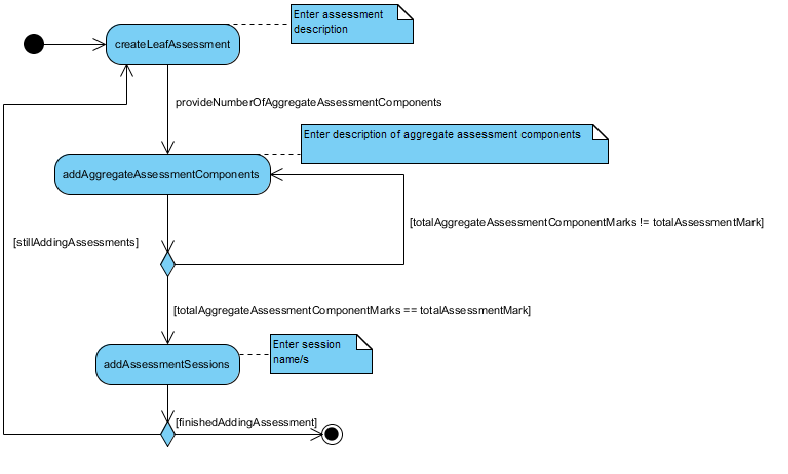
\includegraphics[width=1.0\linewidth, height=12cm]{./Diagrams/uml_assessmentCreation}
		\caption{Activity diagram for creating atomic leaf assessments, aggregate assessments as well as sessions for the atomic assessments.}
		\label{fig:uml_assessmentCreation}
		\end{figure}
	
		The assessment creation operation is only available to lecturers and only has the web interface as shown below.
		
	\pagebreak
	\newpage	
	\subsubsection{Web Interface Screen Designs}
		\begin{figure*}[htbp]
		\centering
		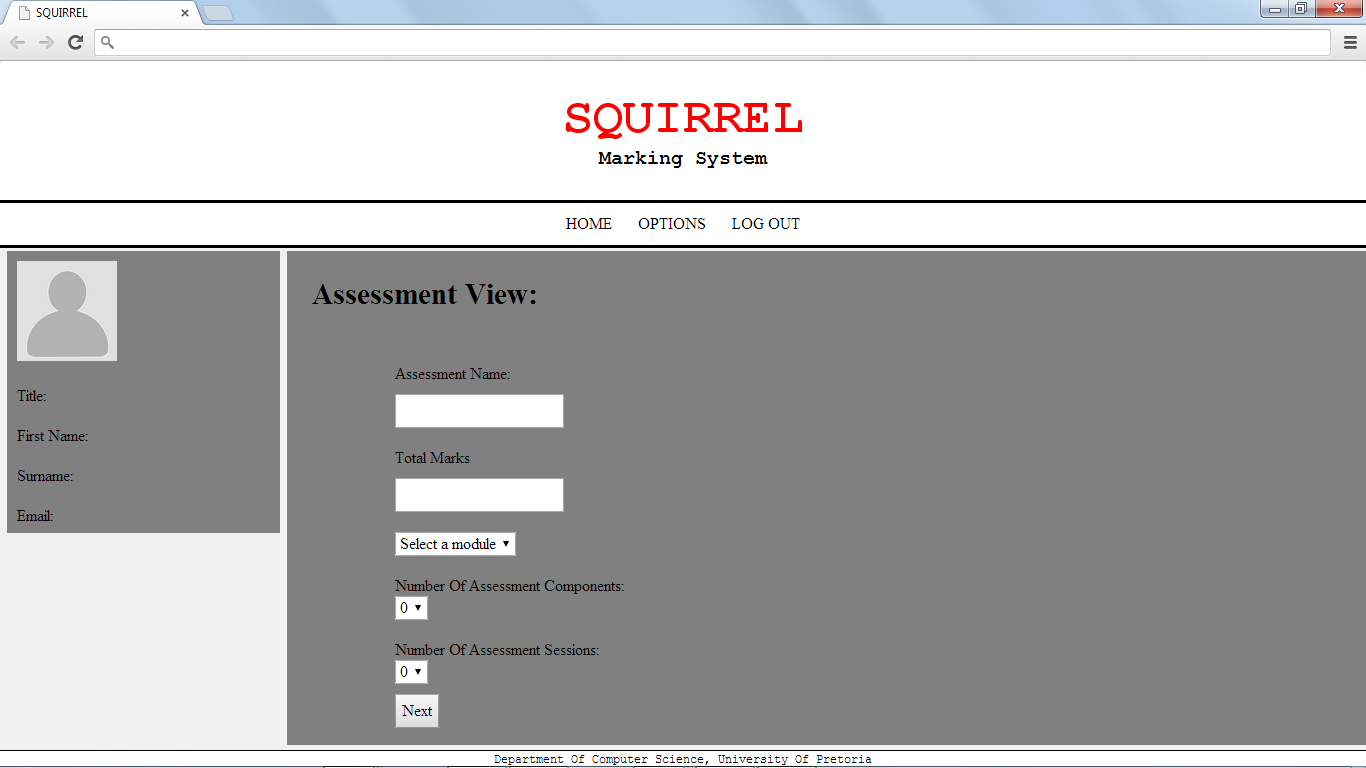
\includegraphics[width=1.0\linewidth,height=12cm]{./Diagrams/web_assessmentView}
		\caption{Screen design for creating an atomic assessment.}
		\label{fig:web_assessmentView}
		\end{figure*}
		
		\begin{figure*}[htbp]
		\centering
		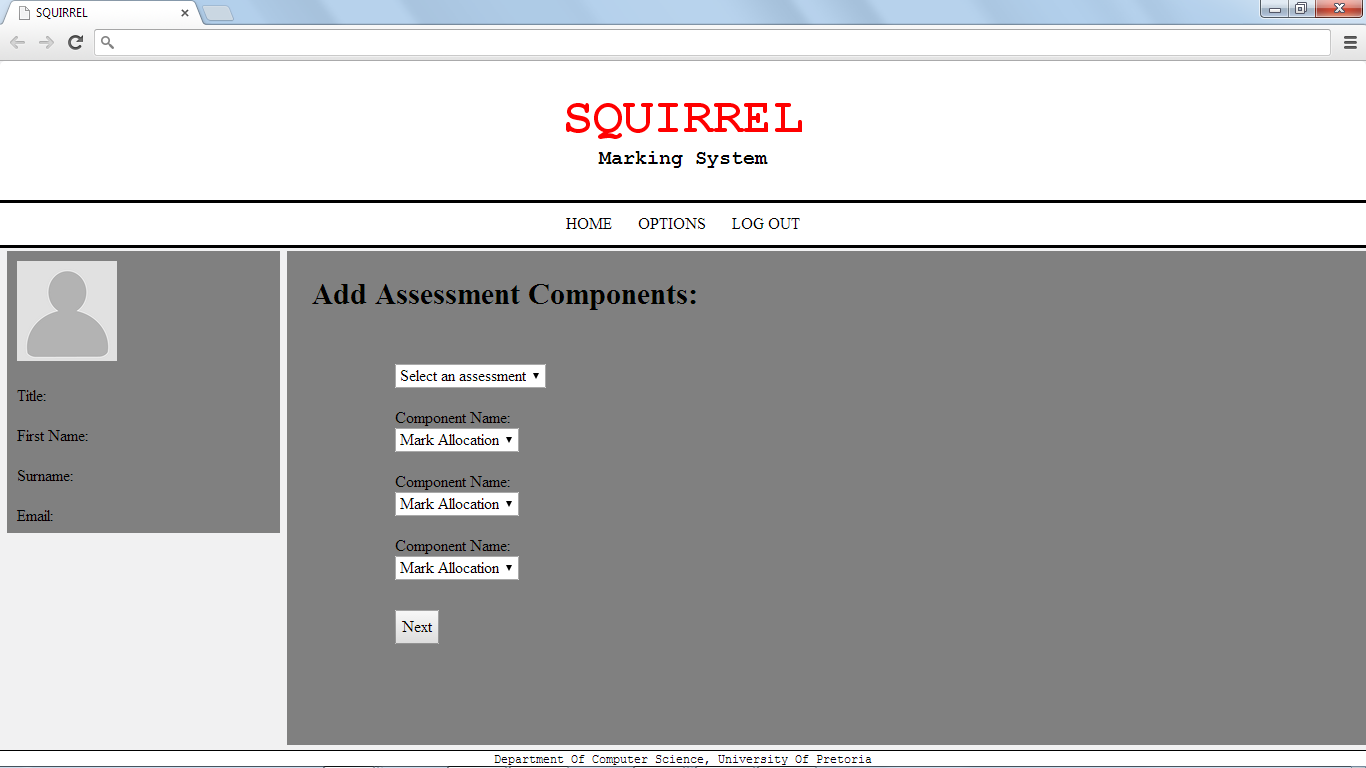
\includegraphics[width=1.0\linewidth, height=12cm]{./Diagrams/web_assessmentComponent}
		\caption{Screen design for adding aggregate assessments.}
		\label{fig:web_assessmentComponent}
		\end{figure*}
	
	\pagebreak
		\begin{figure*}[htbp]
		\centering
		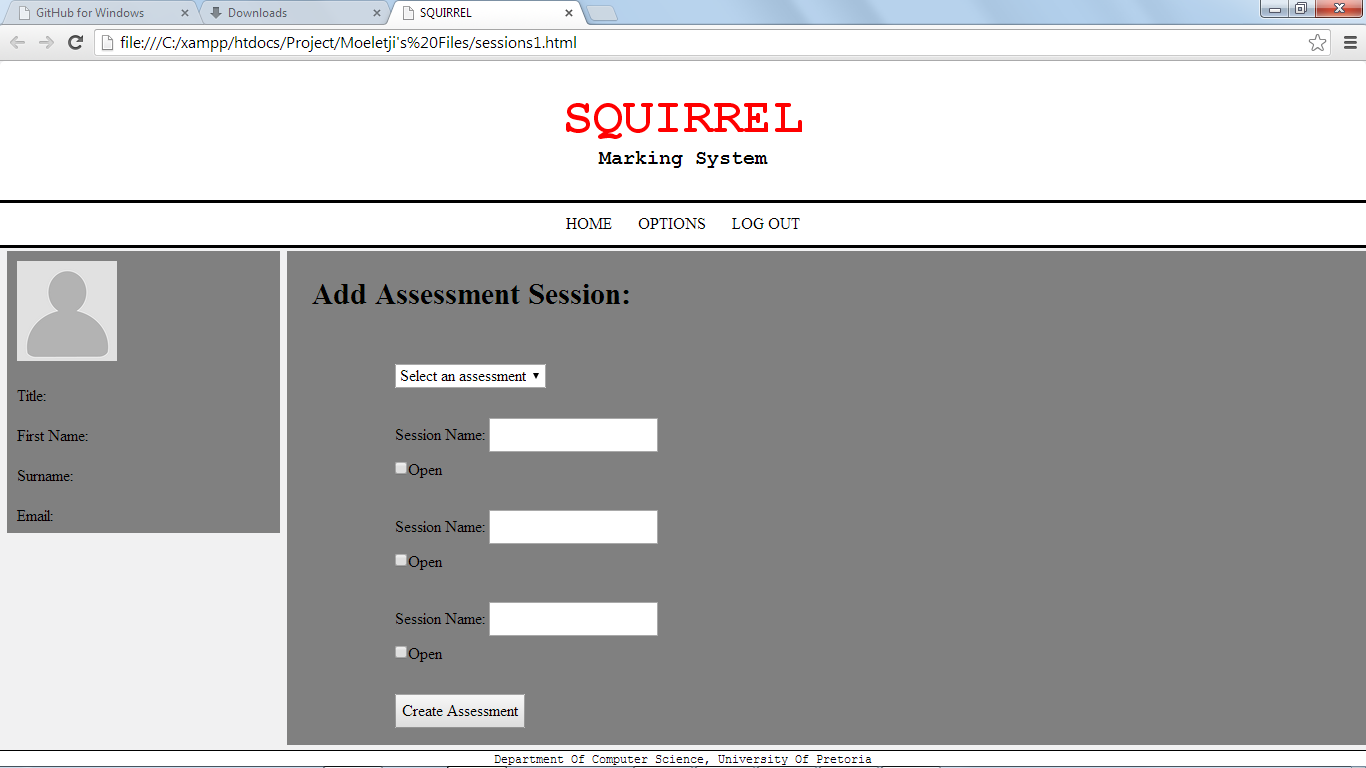
\includegraphics[width=1.0\linewidth, height=12cm]{./Diagrams/web_assessmentSession}
		\caption{Screen design for adding sessions for an atomic assessment.}
		\label{fig:web_assessmentSession}
		\end{figure*}
	
	\newpage
	\subsection{Marks Management}
	
		\begin{figure*}[htbp]
		\centering
		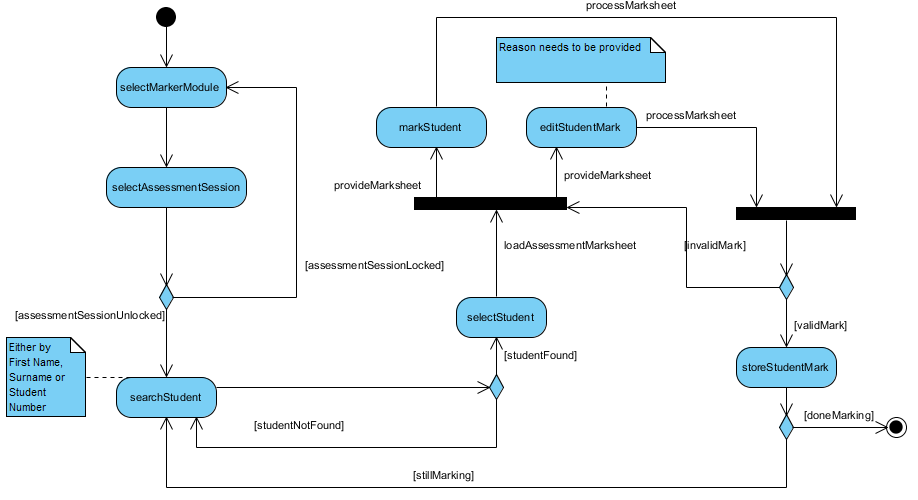
\includegraphics[width=1.0\linewidth, height=12cm]{./Diagrams/uml_markManagement}
		\caption{Activity diagram depiction of how a student would get marked.}
		\label{fig:uml_markManagement}
		\end{figure*}
			
		The activity diagram(Figure 10) depicts how a marker would go about marking a student. The activity diagram is closely linked with the screen designs as it shows how the user would go about marking a student.
	\pagebreak
	
	\subsubsection{Mobile Interface Screen Designs}
	
			\begin{figure*}[htbp]
			\centering
			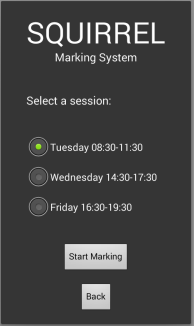
\includegraphics[width=0.7\linewidth, height=12cm]{./Diagrams/mobile_selectSession}
			\caption{Screen design of assessment sessions.}
			\label{fig:mobile_selectSession}
			\end{figure*}
			
	\pagebreak		
		
			\begin{figure*}[htbp]
			\centering
			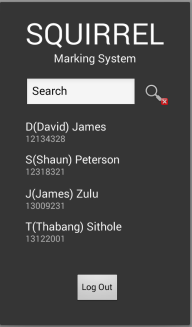
\includegraphics[width=0.7\linewidth, height=12cm]{./Diagrams/mobile_searchForStudent}
			\caption{Screen design of how the students would be displayed and search for on the system.}
			\label{fig:mobile_searchForStudent}
			\end{figure*}
	\pagebreak	
	
			\begin{figure*}[htbp]
			\centering
			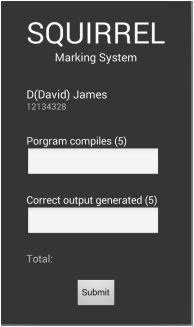
\includegraphics[width=0.7\linewidth, height=12cm]{./Diagrams/mobile_markStudent}
			\caption{Screen design of the interface used to enter student marks.}
			\label{fig:mobile_markStudent}
			\end{figure*}
			
	\pagebreak	
	
	\subsubsection{Web Interface Screen Designs}
	
		\begin{figure*}[htbp]
		\centering
		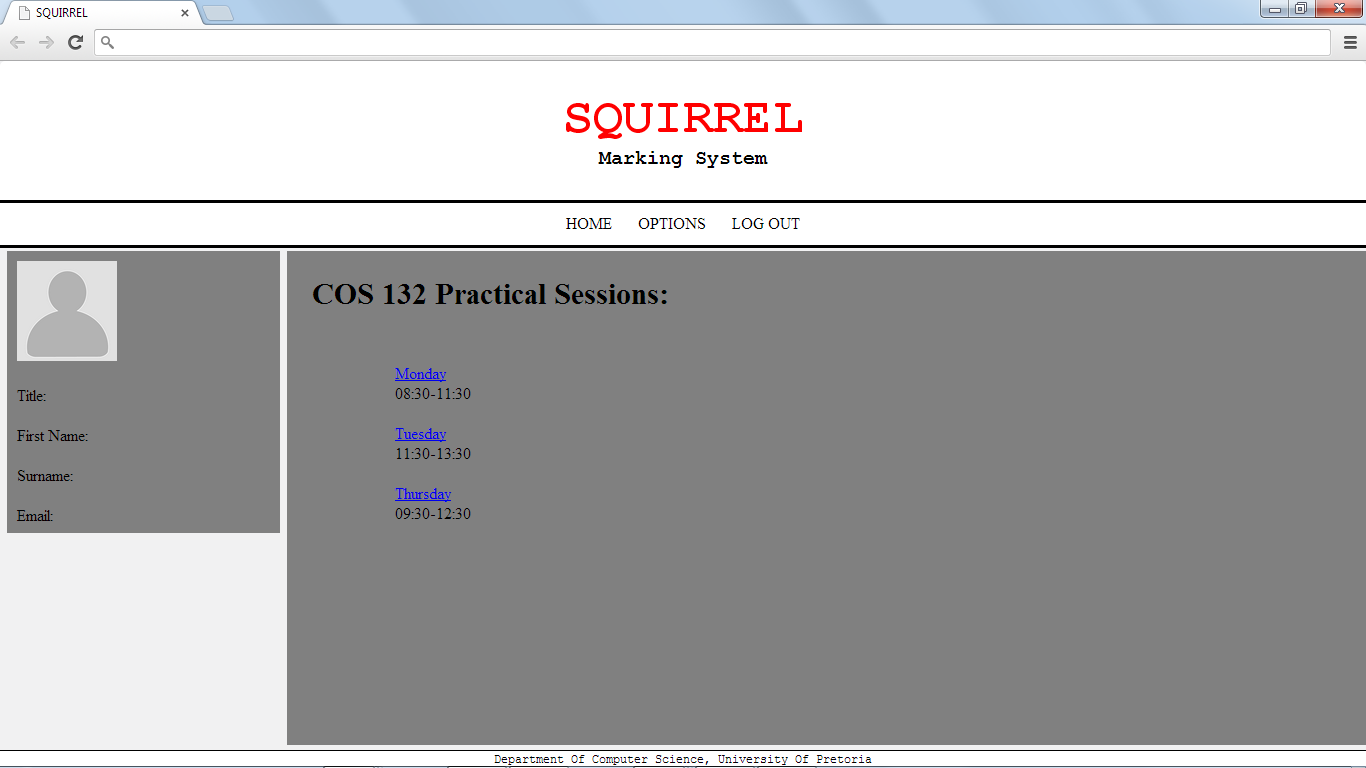
\includegraphics[width=1.0\linewidth, height=12cm]{./Diagrams/web_markerSessions}
		\caption{List of available marking sessions.}
		\label{fig:web_markerSessions}
		\end{figure*}
			
		\begin{figure*}[htbp]
		\centering
		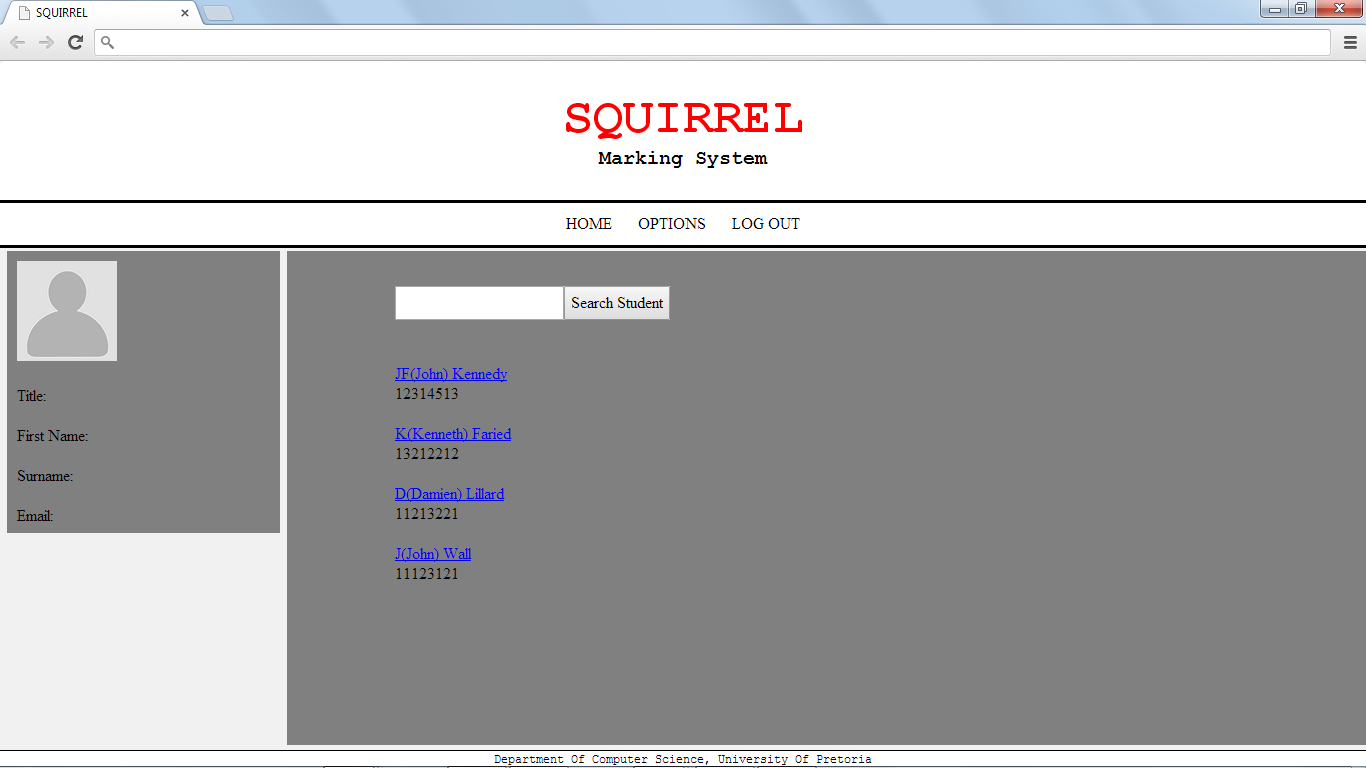
\includegraphics[width=1.0\linewidth, height=12cm]{./Diagrams/web_searchStudent}
		\caption{List of students in the sessions who need to be marked.}
		\label{fig:web_searchStudent}
		\end{figure*}
			
	\pagebreak
		\begin{figure*}[htbp]
		\centering
		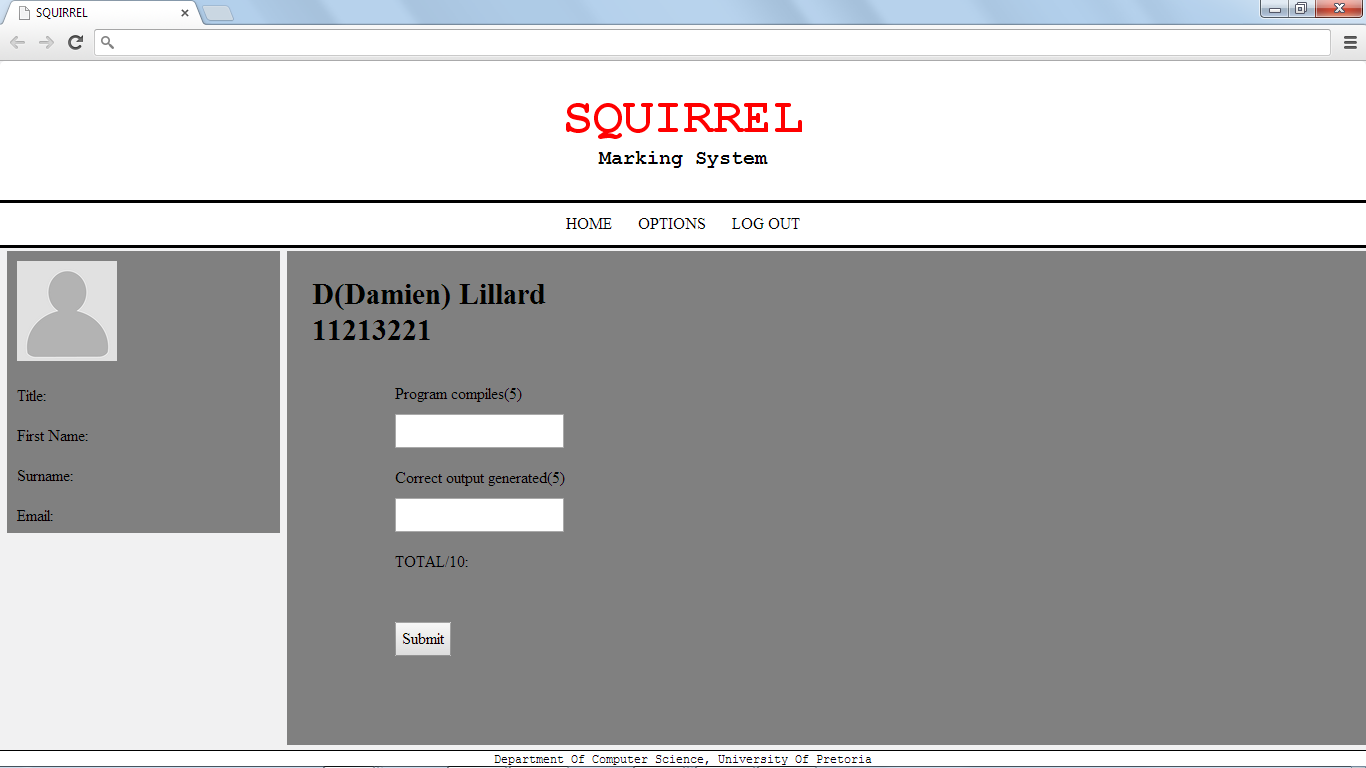
\includegraphics[width=1.0\linewidth, height=12cm]{./Diagrams/web_markStudent}
		\caption{A student being marked.}
		\label{fig:web_markStudent}
		\end{figure*}
	
	\pagebreak
	\newpage
	\subsection{Reporting}
	
		\begin{figure}[htbp]
		\centering
		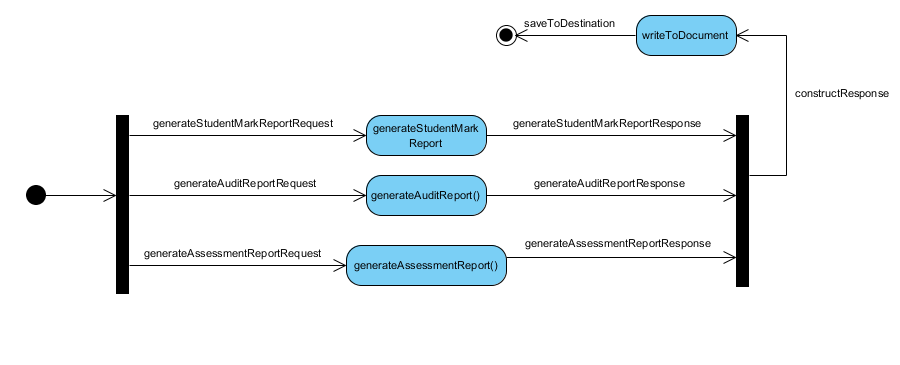
\includegraphics[width=1.0\linewidth, height=12cm]{./Diagrams/uml_reportGenerating}
		\caption{Activity diagram of how reports would be generated by users.}
		\label{fig:uml_reportGenerating}
		\end{figure}
		
		Students wll be able to generate their mark reports on either platform(mobile or web interface), while lecturers will only be able to generate assessment and audit reports via the web interface.
	\pagebreak
	\subsubsection{Mobile Interface Screen Designs}
	
		\begin{figure}[htbp]
		\centering
		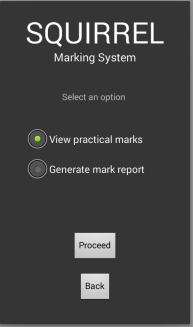
\includegraphics[width=0.7\linewidth, height=12cm]{./Diagrams/mobile_studentViewOption}
		\caption{Options of reports a student can generate.}
		\label{fig:mobile_studentViewOption}
		\end{figure}
	\pagebreak
		\begin{figure}[htbp]
		\centering
		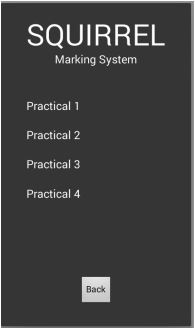
\includegraphics[width=0.7\linewidth, height=12cm]{./Diagrams/mobile_practicalsView}
		\caption{List of practicals.}
		\label{fig:mobile_practicalsView}
		\end{figure}
	
	\clearpage
	\pagebreak
		\begin{figure}[htbp]
		\centering
		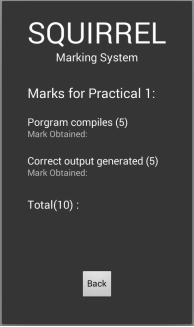
\includegraphics[width=0.7\linewidth, height=12cm]{./Diagrams/mobile_pracMarksheet}
		\caption{Screen design of a report for a students practical 1.}
		\label{fig:mobile_pracMarksheet}
		\end{figure}
	\pagebreak		
		\begin{figure}[htbp]
		\centering
		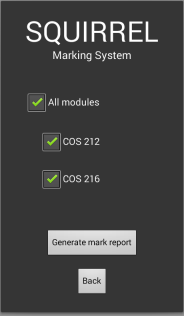
\includegraphics[width=0.7\linewidth, height=12cm]{./Diagrams/mobile_studentReport}
		\caption{Screen design for generating a students' mark report. }
		\label{fig:mobile_studentReport}
		\end{figure}	
	\pagebreak	
	\subsubsection{Web Interface Screen Designs}
	
		\begin{figure*}[htbp]
		\centering
		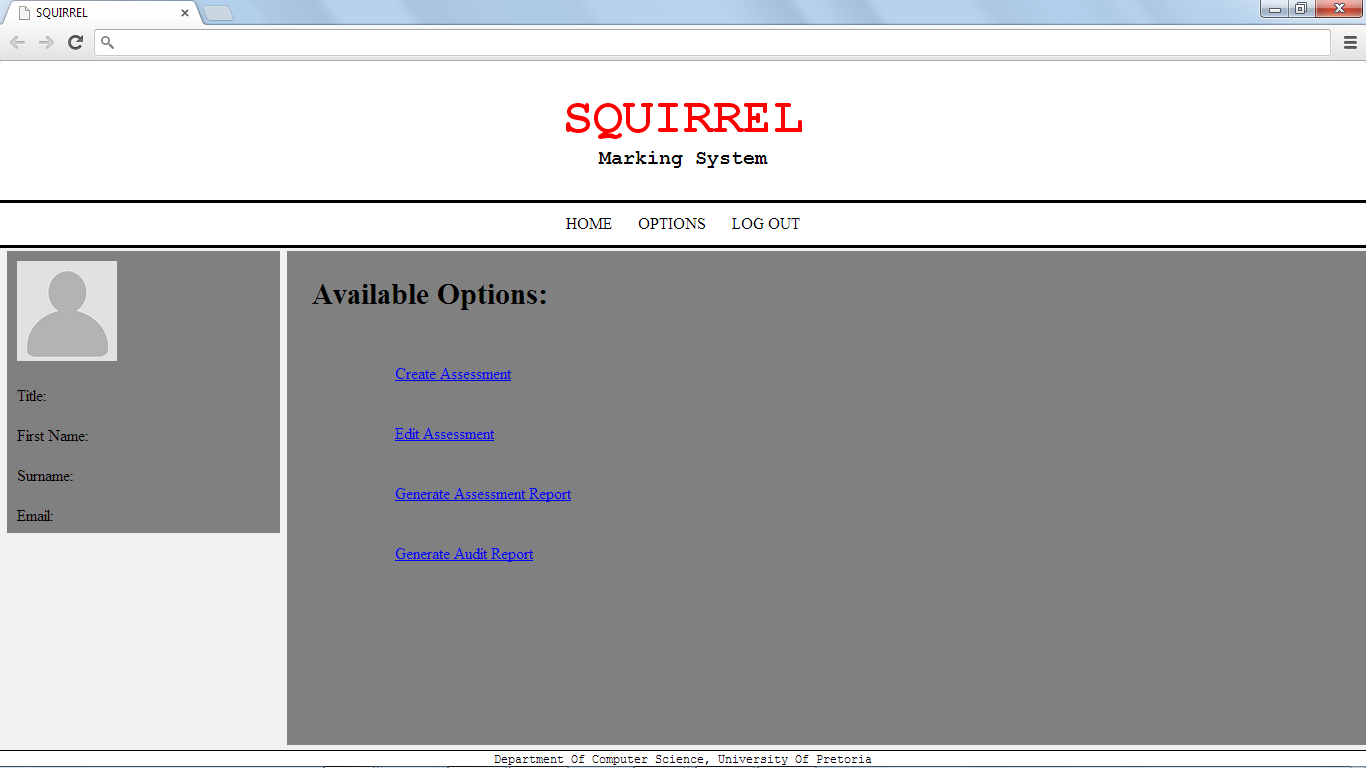
\includegraphics[width=1.0\linewidth, height=12cm]{./Diagrams/web_lecturerOptions}
		\caption{Report options lecturers have.}
		\label{fig:web_lecturerOptions}
		\end{figure*}
	
		\begin{figure*}[htbp]
		\centering
		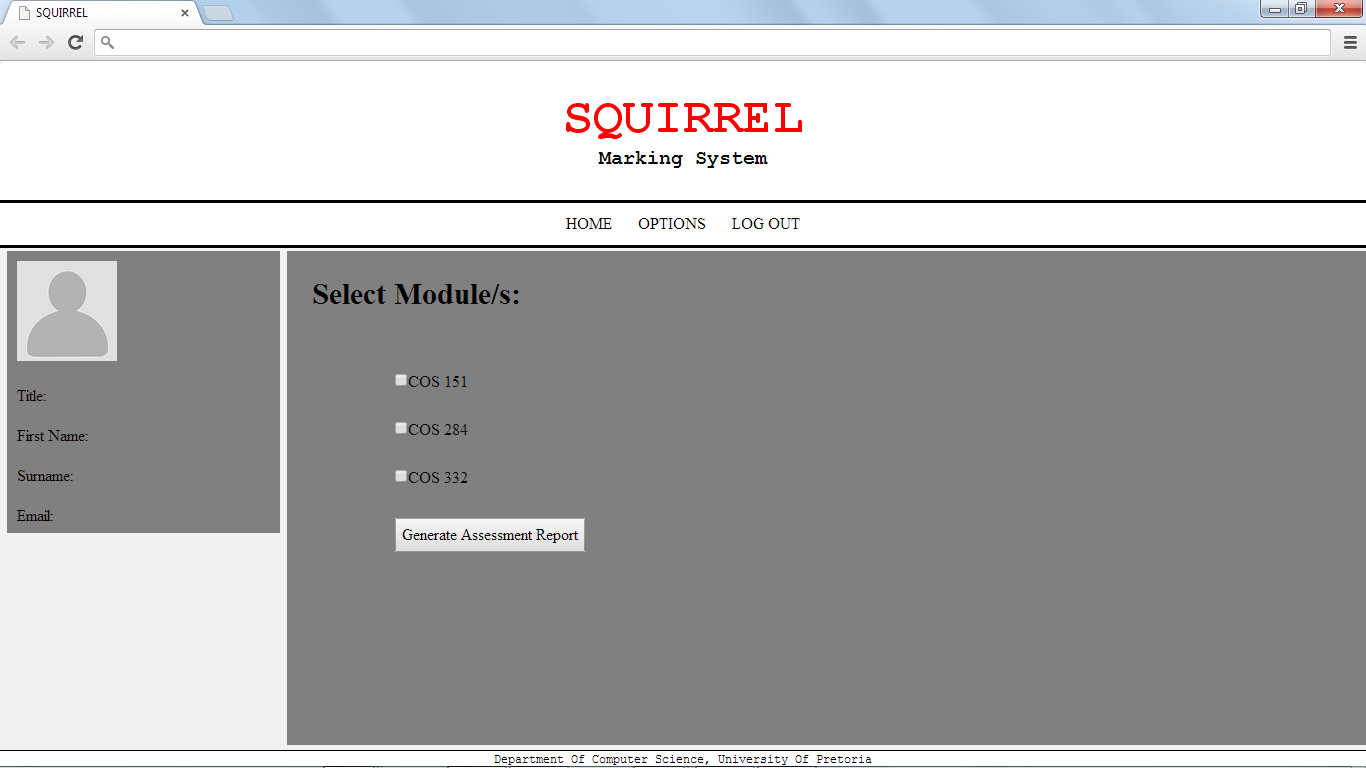
\includegraphics[width=1.0\linewidth, height=12cm]{./Diagrams/web_assessmentReport}
		\caption{Screen design for generating assessment reports.}
		\label{fig:web_assessmentReport}
		\end{figure*}

		\begin{figure}[htbp]
		\centering
		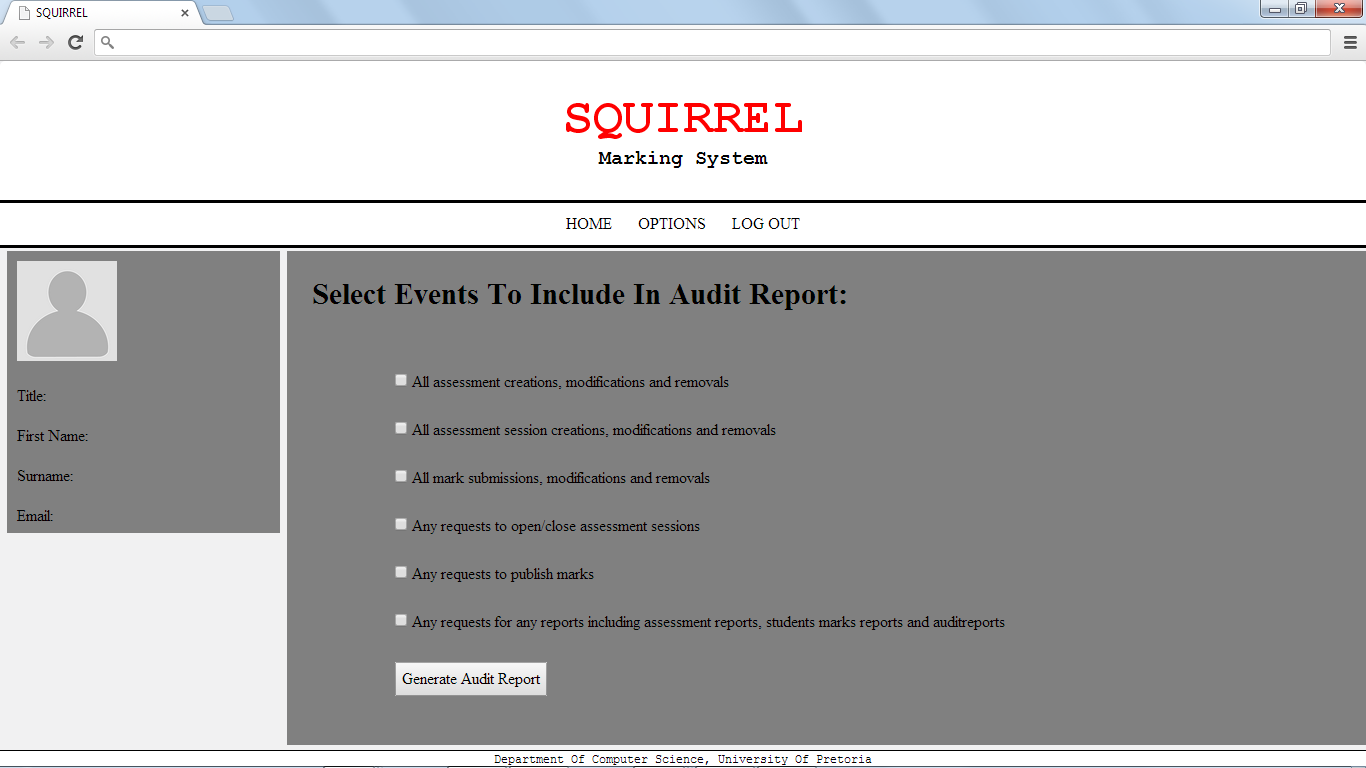
\includegraphics[width=1.0\linewidth, height=12cm]{./Diagrams/web_auditReport}
		\caption{Screen design for generating audit reports.}
		\label{fig:web_auditReport}
		\end{figure}


\end{document}